%%%%%%%%%%%%%%%%%%%%%%%%%%%%%%%%%%%%%%%%%%%%%%%%%%%%%%%%%%%%%%%%%%%%%%
% LaTeX Example: Project Report
%
% Source: http://www.howtotex.com
%
% Feel free to distribute this example, but please keep the referral
% to howtotex.com
% Date: March 2011 
% 
%%%%%%%%%%%%%%%%%%%%%%%%%%%%%%%%%%%%%%%%%%%%%%%%%%%%%%%%%%%%%%%%%%%%%%

\documentclass[paper=letter, fontsize=11pt]{article}
\usepackage[T1]{fontenc}
\usepackage{fourier}

\usepackage[english]{babel}															% English language/hyphenation
%\usepackage[protrusion=true,expansion=true]{microtype}	
\usepackage{amsmath,amsfonts,amsthm} % Math packages
\usepackage[pdftex]{graphicx}	
\usepackage{url}
\usepackage{siunitx}
\usepackage{subfig}
\usepackage{pgf}
\usepackage{float}



%%% Custom sectioning
\usepackage{sectsty}
\allsectionsfont{ \normalfont\scshape}


%%% Custom headers/footers (fancyhdr package)
\usepackage{fancyhdr}
\pagestyle{fancyplain}
\fancyhead{}											% No page header
\fancyfoot[L]{}											% Empty 
\fancyfoot[C]{}											% Empty
\fancyfoot[R]{\thepage}									% Pagenumbering
\renewcommand{\headrulewidth}{0pt}			% Remove header underlines
\renewcommand{\footrulewidth}{0pt}				% Remove footer underlines
\setlength{\headheight}{13.6pt}


%%% Equation and float numbering
\numberwithin{equation}{section}		% Equationnumbering: section.eq#
\numberwithin{figure}{section}			% Figurenumbering: section.fig#
\numberwithin{table}{section}				% Tablenumbering: section.tab#


%%% Maketitle metadata
\newcommand{\horrule}[1]{\rule{\linewidth}{#1}} 	% Horizontal rule

\title{
		%\vspace{-1in} 	
		\usefont{OT1}{bch}{b}{n}
		\normalfont \normalsize \textsc{State University at Buffalo} \\ [25pt]
		\horrule{0.5pt} \\[0.4cm]
		\Large Homework3 : Clustering Analysis for Complex Networks \\
		\horrule{2pt} \\[0.5cm]
}
\author{
		\normalfont\large 								
        Yuze Liu \hspace{1.2cm}50207903\\
        \normalfont\large 
        Luting Chen \hspace{0.5cm}50133507\\
        \normalfont\large 
        Vicky Zheng \hspace{0.5cm}50037709\\
}
\date{\large 11/29/2016}
%%% Begin document
\begin{document}
\maketitle
%\newdimen\origiwspc%
\section{Introduction of MCL Algorithm}
MCL Algorithm is The Markov Cluster Algorithm. It is a graph clustering algorithm. In the graph, each vertex is connected to others by weighted or unweighted edges. MCL is based on Random Walks, start at a arbitrary node and then randomly travel to connected node, it will be more likely to stay within a cluster than travel between them. So bby doing random walks upon the graph, it is possible to discover the clusters in the graph.
\section{Implementation}
The MCL I implemented is based on the following algorithm which is provided in the class:
\begin{enumerate}
	\item Input is an un-directed graph, power parameter k, and inflation parameter r.
	\item Create the associated matrix.
	\item Add self loops to each matrix.
	\item Normalize the matrix.
	\item Expand by taking the $k^{th}$ power of the matrix.
	\item Inflate by taking inflation of the resulting matrix with parameter r.
	\item Repeat steps 5 and 6 until a steady state is reached.
	\item Interpret resulting matrix to discover clusters.
\end{enumerate}
In my implementation, I used python 2.7, sklearn packag has been used to normalize the matrix. The iterations is set as 100 times, which turns out that for the given data, after 100 times iteration, the steady state will always be reached, and it won't take more than 5 seconds.\\
In order to show the best result, the Pajek is used to visualize the clusters. By trying with different value of k and r, the clusters are also different. Basically, with k increasing, the number of the clusters will decrease and with r increase, the number of clusters will also increase.
\section{Visualization of the 3 given dataset}
Three dataset has been given for testing the algorithm. After trying with different, the most reasonable result and the related parameters are shown below.\\
Dataset1 attweb\_net :\\
k = 3, r = 2, clusters : 6\\
\begin{figure}[H]
	\centering
	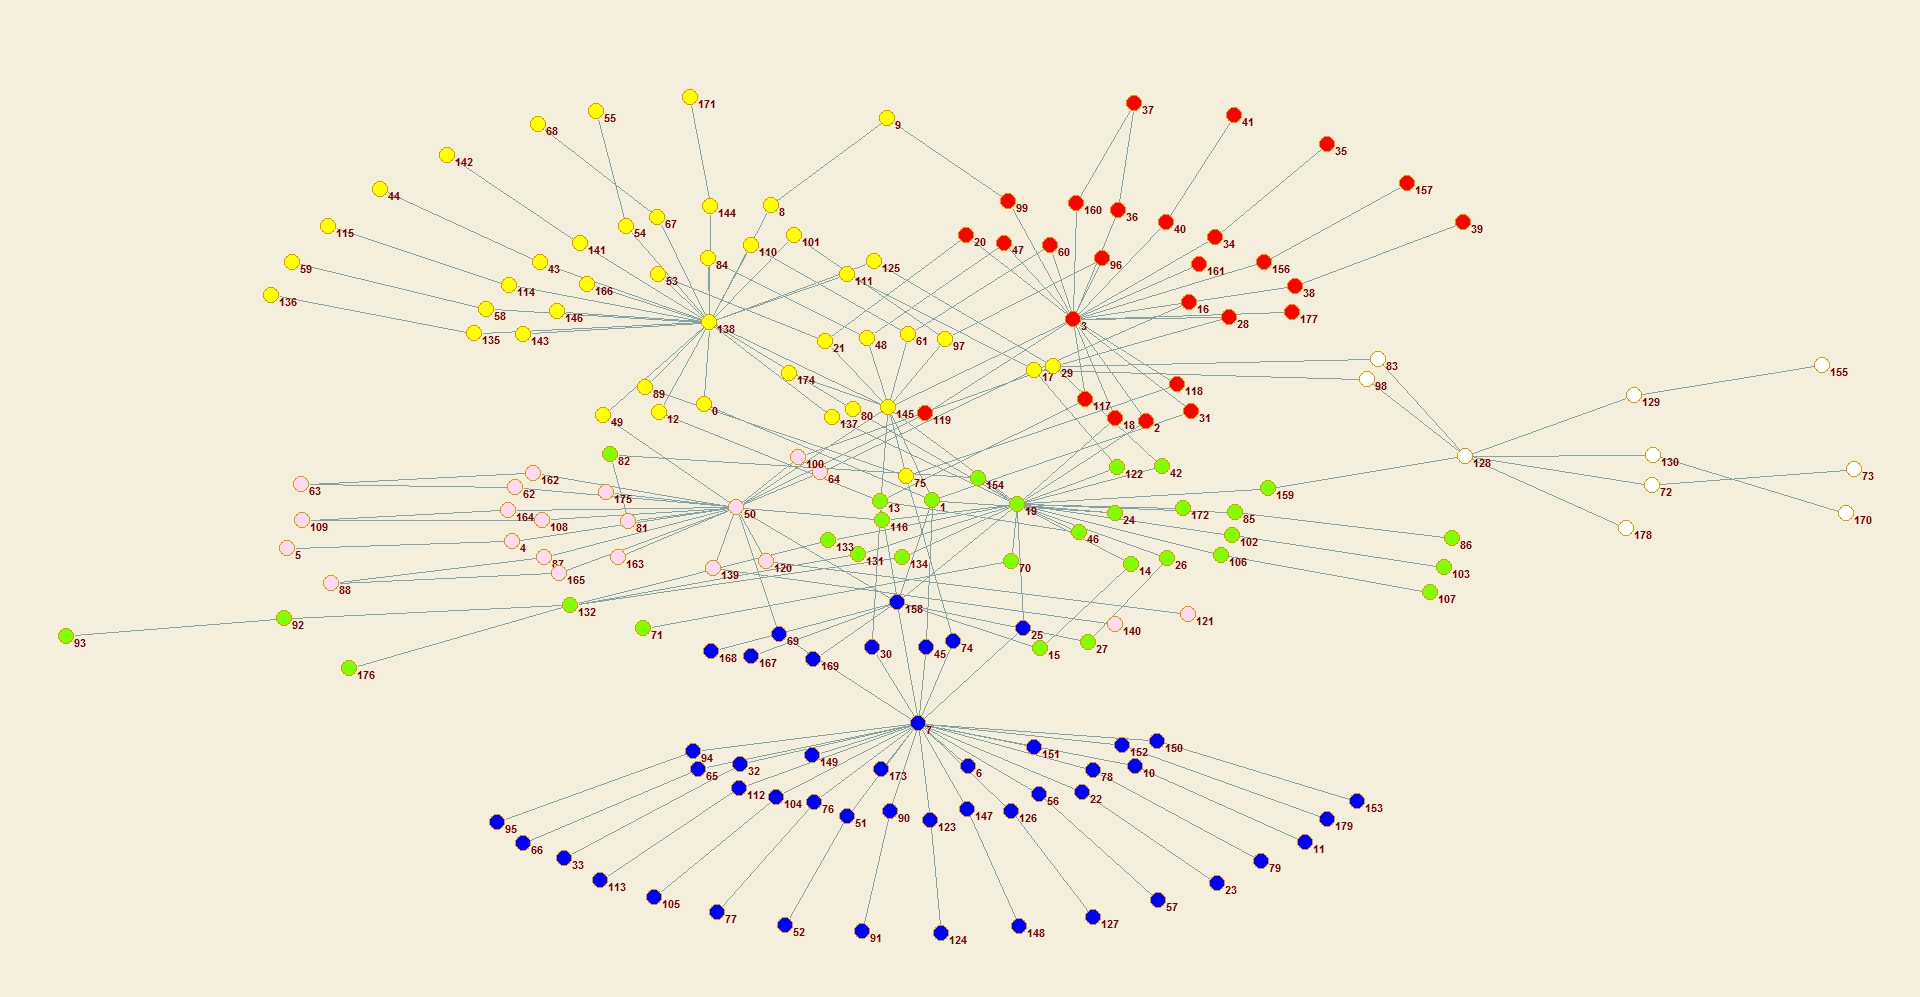
\includegraphics[width=1\textwidth]{attweb_net_6.jpg}
	\caption{Result of attweb\_net graph 2D Version,k = 3, r = 2, clusters = 6}
\end{figure}
Dataset2 physics\_collaboration\_net :\\
k = 7, r = 7, clusters : 5\\
\begin{figure}[H]
	\centering
	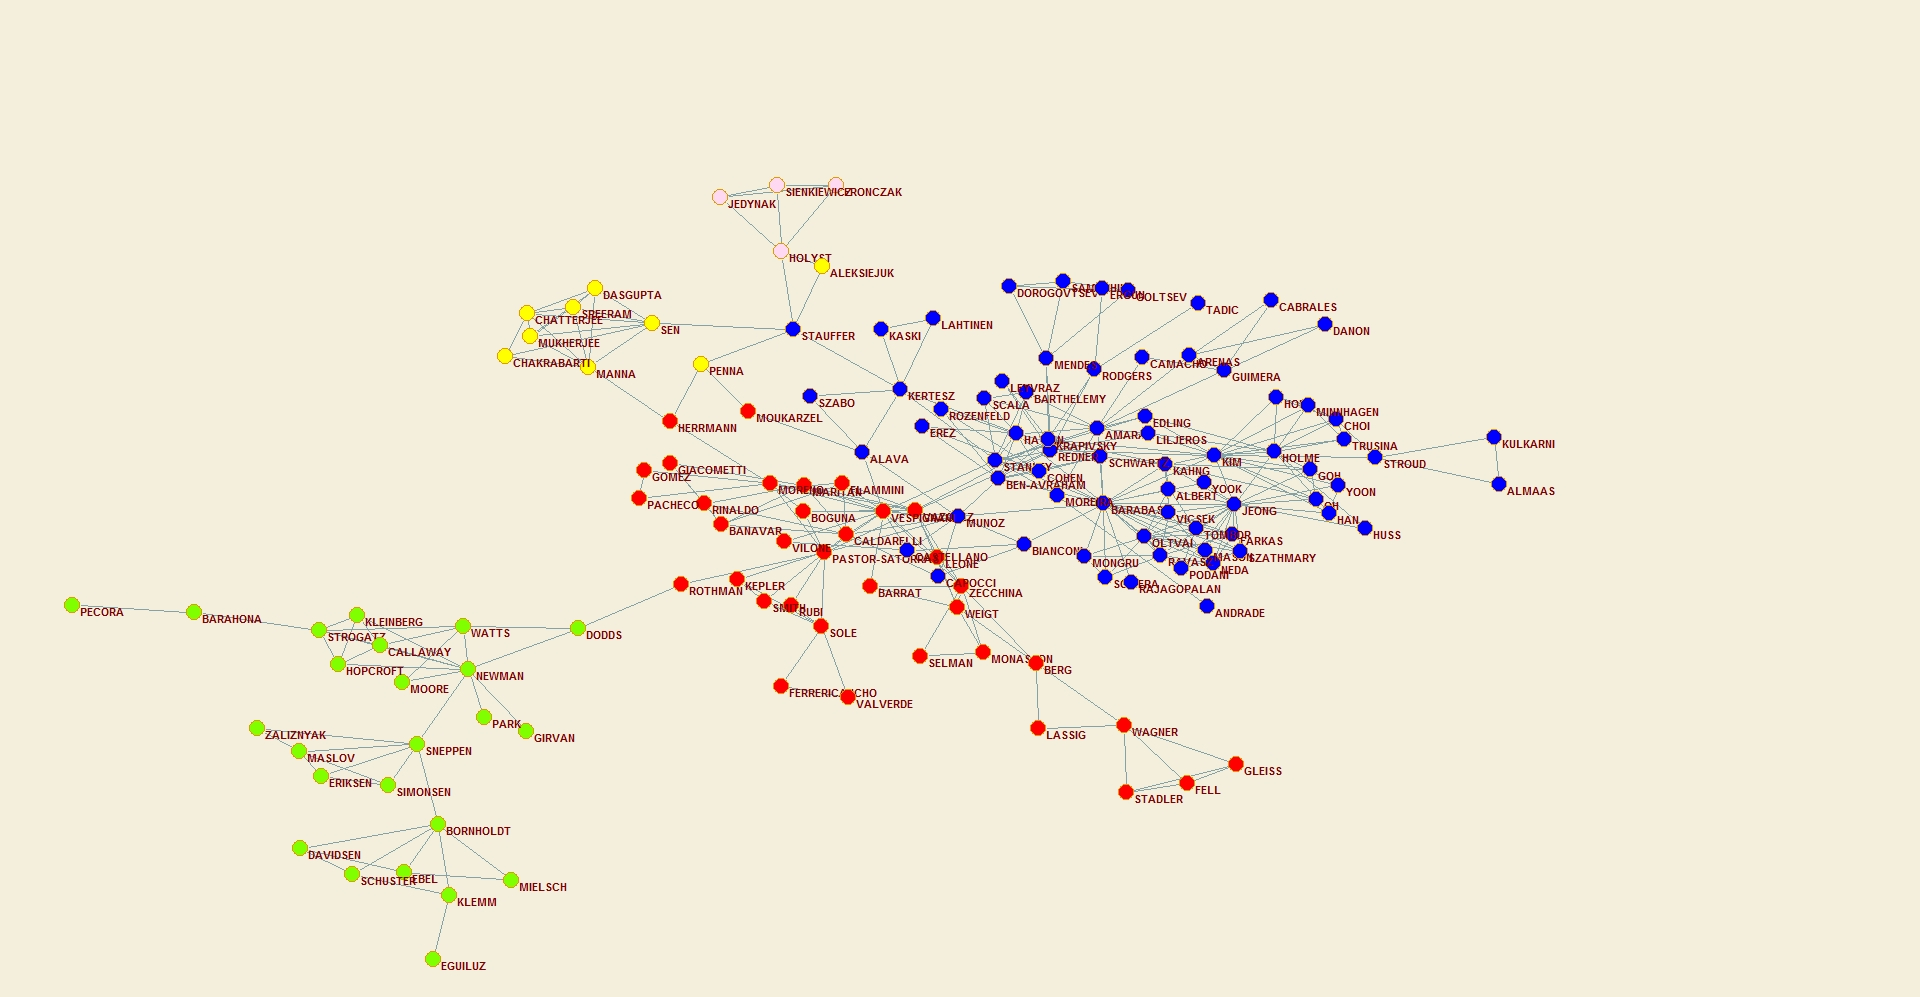
\includegraphics[width=1\textwidth]{physics_c5_k7_r7.jpg}
	\caption{Result of physics\_collaboration\_net 2D Version,k = 7, r = 7, clusters = 5}
\end{figure}
Dataset3 yeast\_undirected\_metabolic :\\
k = 10, r = 3, clusters : 9\\
\begin{figure}[H]
	\centering
	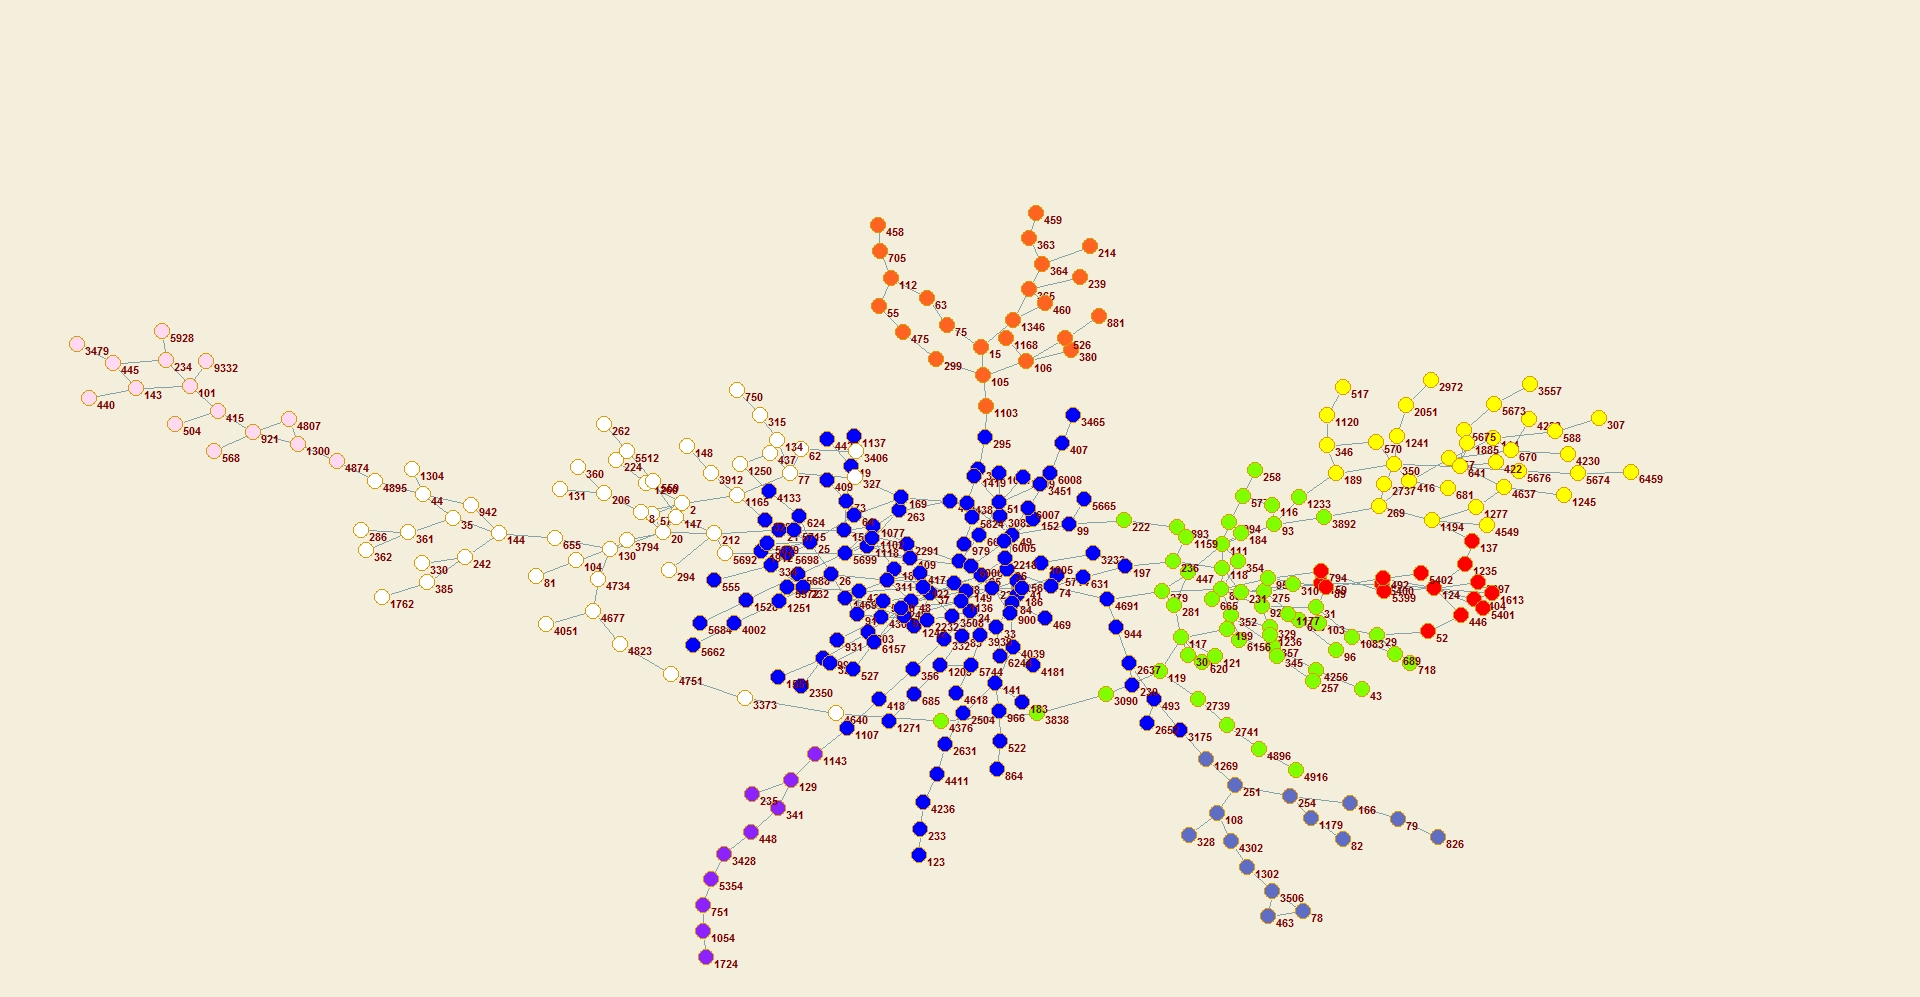
\includegraphics[width=1\textwidth]{yeast_c9_k10_r3.jpg}
	\caption{Result of yeast\_undirected\_metabolic graph 2D Version,k = 10, r = 3, clusters = 9}
\end{figure}


\end{document}